\documentclass[11pt]{article}
\usepackage[margin=1in]{geometry}
\usepackage{amsmath,amssymb,amsthm,bm}
\usepackage{booktabs,array}
\usepackage[most]{tcolorbox}
\usepackage{tikz}
\usetikzlibrary{arrows.meta,positioning,shapes.geometric,calc,fit,backgrounds,decorations.pathreplacing}
\usepackage{pgfplots}
\pgfplotsset{compat=1.18}
\usepackage{algorithm}
\usepackage{algpseudocode}
\usepackage{hyperref}
\usepackage{xcolor}
\hypersetup{colorlinks=true,linkcolor=blue!50!black,citecolor=blue!50!black,urlcolor=blue!50!black}

% ---- three-level boxes -------------------------------------------------
\newtcolorbox{eli}{colback=green!5,colframe=green!45!black,title=ELI5,fonttitle=\bfseries,breakable}
\newtcolorbox{intu}{colback=blue!4,colframe=blue!45!black,title=Intuition,fonttitle=\bfseries,breakable}
\newtcolorbox{rig}{colback=gray!6,colframe=black!70,title=Rigor,fonttitle=\bfseries,breakable}
\newtcolorbox{warn}{colback=orange!6,colframe=orange!70!black,title=Where it breaks / what is assumed,fonttitle=\bfseries,breakable}

% ---- tikz styles --------------------------------------------------------
\tikzset{
  box/.style={draw,rounded corners,align=center,minimum height=8mm,inner sep=4pt,fill=white},
  data/.style={draw,align=center,inner sep=4pt,fill=yellow!12,rounded corners=1pt,font=\small\ttfamily},
  gate/.style={draw,diamond,aspect=2.2,align=center,inner sep=1pt,fill=orange!10,font=\small},
  proc/.style={box,fill=blue!6},
  ext/.style={box,fill=green!8},
  arr/.style={-{Latex[length=2mm]},thick},
  lbl/.style={font=\scriptsize,fill=white,inner sep=1pt}
}

\newcommand{\lv}{\lambda_v}\newcommand{\lr}{\lambda_r}\newcommand{\lm}{\lambda_m}
\newcommand{\tf}{t_f}\newcommand{\R}{\mathbb{R}}
\newcommand{\file}[1]{\texttt{#1}}
\newcommand{\Qmt}{Q_{mt}}

\title{Algorithms for Optimal Low-Thrust Orbit Transfers in the Earth--Moon CR3BP:\\
Min-Time, Min-Energy, Min-Fuel --- how we solve them, how data flows, how we verify}
\author{M.~Casey \quad (Coorbital orbit-transfer library, \file{orbit\_transfer/})}
\date{2026-09-07 \quad (review draft)}

\begin{document}
\maketitle

\begin{abstract}
This document is the algorithmic companion to the orbit-transfer code base. It
states the goal --- minimum-time, minimum-energy and minimum-fuel low-thrust
transfers between periodic orbits of the Earth--Moon circular restricted
three-body problem --- writes the optimal control problem once, explicitly,
and then follows the two solution lines the library actually runs:
the \emph{min-time} line (direct collocation $\to$ covector harvest $\to$
multiple shooting $\to$ acceptance $\to$ catalog) and the \emph{min-fuel} line
(min-energy at fixed final time $\to$ a homotopy walk to min-fuel through one
of three smoothing families, including the PLQ/Huber family and its
continuous hybrid). Every algorithm is presented three times: as a
one-paragraph picture (ELI5), as the reasoning an engineer needs to trust it
(Intuition), and as the equations and loops the code implements (Rigor).
Flow diagrams show where data enters, what each stage produces, and which
files carry it. A final chapter separates what the verification layer
\emph{proves} from what it \emph{assesses}. Numbers quoted are the measured
ones in \file{DRO\_tulip/FINDINGS.md}.
\end{abstract}

\tableofcontents

%======================================================================
\section{The goal and the problem}
%======================================================================

\subsection{Goal}
Given a departure periodic orbit (DRO, halo, DPO, \ldots) and an arrival
periodic orbit (a tulip orbit, or another halo), both in the Earth--Moon
rotating frame, and a spacecraft with a fixed low-thrust engine, find the
thrust program that moves the spacecraft from a chosen point on the first
orbit to a chosen point on the second while minimizing one of
\begin{center}
\begin{tabular}{@{}lll@{}}
\toprule
objective & minimizes & role in the library \\
\midrule
\textbf{min-time}  & $\tf$ & the four costate catalogs (18,360 entries) consumed by \file{pumpkyn.cr3bp.tfMin} \\
\textbf{min-energy} & $\int_0^{\tf} s^2\,dt$ at fixed $\tf$ & the smooth \emph{starting point} of the fuel line, never a deliverable by itself \\
\textbf{min-fuel}   & $\int_0^{\tf} s\,dt$ at fixed $\tf$ (equivalently, maximize $m(\tf)$) & the min-fuel catalog (18 entries, $\gamma$ up to 2) \\
\bottomrule
\end{tabular}
\end{center}
and, for every solution, say how well we know it is optimal.

\begin{eli}
A spacecraft with a very weak engine (0.07--15 N pushing 150 kg: like blowing on
a bowling ball) has to get from one loop around the Moon to another. It can
point its engine any direction and run it anywhere between off and full. We
want either the fastest trip, or --- if the trip length is fixed --- the one
that burns the least propellant. Fastest means ``engine on the whole way,
point it well.'' Least propellant means ``engine either full on or fully off,
never in between, and switch at exactly the right moments.'' Finding \emph{when}
to switch is the whole difficulty.
\end{eli}

\subsection{Dynamics and control}
Nondimensional CR3BP units (length $L^\star$ = Earth--Moon distance, time
$T^\star$ = $1/n$; the constants sit in \file{cr3bp\_lt\_params}). State
$x=(r,v,m)\in\R^7$; control $u=(\alpha,s)$ with $\alpha\in S^2$ the thrust
direction and $s\in[0,1]$ the throttle:
\begin{equation}\label{eq:dyn}
\dot r = v,\qquad
\dot v = g(r) + h(v) + \frac{sT}{m}\alpha,\qquad
\dot m = -\frac{sT}{c},
\end{equation}
with $g(r)$ the gravity of both primaries plus the centrifugal term,
$h(v)=(2v_y,-2v_x,0)$ the Coriolis term, $T$ the thrust acceleration at unit
mass fraction, $c$ the exhaust velocity ($c = I_{sp}g_0$ in ND). Mass is a
fraction: $m(0)=1$.

\subsection{The optimal control problem, once}
\begin{rig}
\begin{align}
\min_{\alpha(\cdot),\,s(\cdot),\,(\tf)}\quad & J = \phi(\tf) + \int_0^{\tf} L(s)\,dt \label{eq:J}\\
\text{s.t.}\quad & \eqref{eq:dyn},\qquad \alpha(t)\in S^2,\quad s(t)\in[0,1],\notag\\
& r(0)=r_0,\ v(0)=v_0,\ m(0)=1,\qquad r(\tf)=r_f,\ v(\tf)=v_f,\qquad m(\tf)\ \text{free},\notag
\end{align}
with
\[
\begin{array}{lll}
\text{min-time:}   & \phi=\tf,\ L=0,\ \tf\ \text{free} & (\text{equivalently } L=1,\ \phi=0)\\
\text{min-energy:} & \phi=0,\ L=s^2,\ \tf=\gamma\,\tf^{\min}\ \text{fixed} & \gamma>1\\
\text{min-fuel:}   & \phi=0,\ L=s,\ \tf=\gamma\,\tf^{\min}\ \text{fixed} &
\end{array}
\]
$\tf^{\min}$ is the min-time value for the same endpoints; $\gamma$ is the
time-of-flight multiplier (the catalog's third axis).
\end{rig}

\subsection{Pontryagin's principle, once}
\begin{intu}
The maximum principle turns ``choose a whole control history'' into
``choose seven numbers.'' It introduces a costate $\lambda=(\lr,\lv,\lm)$ ---
the sensitivity of the optimal cost to the state, a shadow price --- that
obeys its own differential equation, and it says the optimal control at each
instant is the one that minimizes a scalar function $H$ of the current state
and costate. So once $\lambda(0)$ is known, the entire trajectory follows by
integrating an ODE. The seven unknowns $\lambda(0)$ (plus $\tf$ when free) are
fixed by the seven (eight) end conditions. Everything in this document is a
way of solving that root-finding problem well, and of checking the root.
\end{intu}
\begin{rig}
With the normal multiplier $\lambda_0=1$,
\begin{equation}\label{eq:H}
H = L(s) + \lr\!\cdot v + \lv\!\cdot\big(g(r)+h(v)\big) + sT\Big(\frac{\lv\!\cdot\alpha}{m}-\frac{\lm}{c}\Big).
\end{equation}
\textbf{Costate equations} $\dot\lambda=-\partial H/\partial x$:
\begin{equation}\label{eq:costate}
\dot\lr = -\big(\partial_r g\big)^{\!\top}\lv,\qquad
\dot\lv = -\lr - \big(\partial_v h\big)^{\!\top}\lv,\qquad
\dot\lm = \frac{sT}{m^2}\,|\lv| .
\end{equation}
\textbf{Minimum condition.} Over $\alpha\in S^2$: $\alpha^*=-\lv/|\lv|$ (the
primer direction; requires $|\lv|\ne0$). Over $s\in[0,1]$, $H$ is
$L(s)-sQ$ plus terms without $s$, where
\begin{equation}\label{eq:Q}
Q := T\Big(\frac{|\lv|}{m}+\frac{\lm}{c}\Big)
\end{equation}
is the \emph{switch quantity}. The throttle law is $s^*=\arg\min_{[0,1]}\big(L(s)-sQ\big)$:
\[
\begin{array}{ll}
\text{min-time (}L\equiv1\text{ or }0\text{):} & s^*=1 \text{ iff } Q>0 \ (\text{all-burn; } Q>0 \text{ is checked, \S\ref{sec:mt-verify}}),\\
\text{min-energy (}L=s^2\text{):} & s^*=\mathrm{clip}(Q/2,\,0,\,1),\\
\text{min-fuel (}L=s\text{):} & s^*=1 \text{ if } Q>1,\ 0 \text{ if } Q<1 \quad(\text{bang-bang}).
\end{array}
\]
\textbf{Transversality.} $m(\tf)$ free $\Rightarrow \lm(\tf)=0$. $\tf$ free
(min-time) $\Rightarrow H(\tf)=0$, hence $H\equiv0$ along the arc (autonomous
system). Fixed $\tf$ $\Rightarrow$ $H\equiv$ const (used as a check).
\end{rig}

\begin{eli}
$Q$ is a single dial that the physics computes for you at every instant.
For the fuel problem the rule is childishly simple: dial above 1, engine on;
dial below 1, engine off. The hard part is that the dial's reading depends on
the seven starting numbers you have to guess.
\end{eli}

\paragraph{What differs between the three objectives.} Only $L(s)$ and the
$\tf$ condition. The dynamics, the costate equations, the primer direction, the
switch quantity $Q$ and the free-mass transversality are shared. This is why one
engine (\file{ms\_bvp}) and one propagator family serve all three.

%======================================================================
\section{The data model}
%======================================================================
Every algorithm below manipulates a small number of objects. Naming them once
avoids confusion later.

\begin{center}\small
\begin{tabular}{@{}llp{0.55\textwidth}@{}}
\toprule
object & shape & meaning \\
\midrule
$y$ & $14\times1$ & the augmented state $[r;v;m;\lr;\lv;\lm]$ --- what every propagator integrates \\
$z_8$ & $8\times1$ & a \textbf{min-time} solution: $[\lambda(0);\ \tf]$ in \file{tfMin}'s convention; the catalog entry \\
$\lambda_0$, $Y_j$ & $7\times1$, $14\times(K{+}1)$ & a \textbf{fixed-$\tf$} solution: the initial costate and the $K{+}1$ junction states of the multiple-shooting mesh (the ``identifiability rule'': ship the junctions, not just $\lambda_0$) \\
seed & struct & $\{\tf, \mathrm{tGrid}\,[1{\times}K{+}1], Y\,[14{\times}K{+}1]\}$ --- the multiple-shooting input contract \\
$\Phi(t,0)$ & $14\times14$ & state transition matrix of the PMP flow (variational equations integrated with $y$) \\
record & struct & one (cell, $\gamma$) of the fixed-$\tf$ line: endpoints, $\tf$, $\lambda_0$, $K$, gates \\
sheet & struct & one (departure orbit, arrival orbit) pair: 3-D grids over (departure phase, arrival phase, thrust or $\gamma$) \\
\bottomrule
\end{tabular}
\end{center}

A \textbf{cell} is a (departure phase, arrival phase) pair on the $12\times12$
phasing torus of one sheet; \emph{(2,5)}, \emph{(6,8)}, \emph{(1,2)} are the
three flagship cells of the fixed-$\tf$ line.

%======================================================================
\section{Min-time: the catalog pipeline}
%======================================================================

\begin{figure}[t]\centering
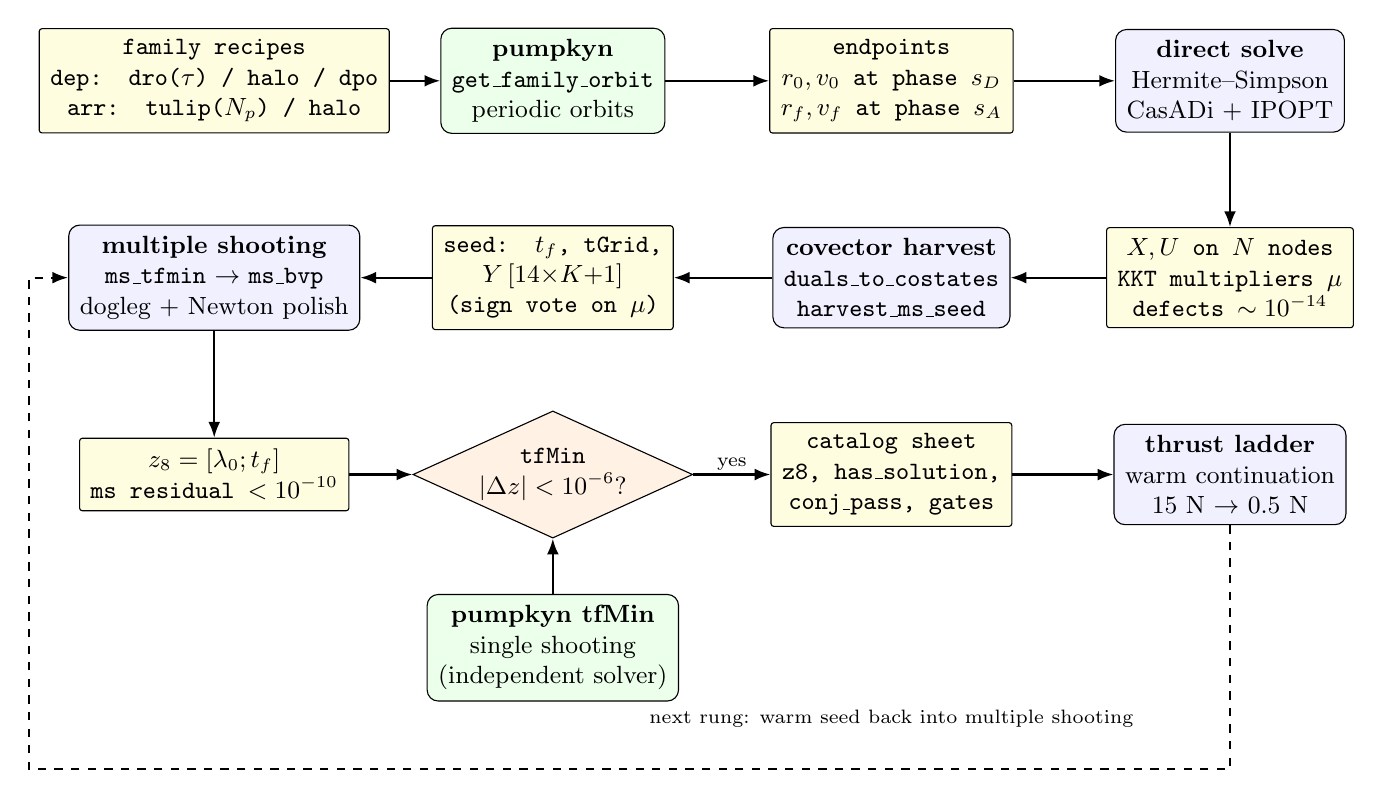
\begin{tikzpicture}[font=\small]
\node[data] (orb) at (0,0) {family recipes\\dep: dro($\tau$) / halo / dpo\\arr: tulip($N_p$) / halo};
\node[ext] (pump) at (4.3,0) {\textbf{pumpkyn}\\\texttt{get\_family\_orbit}\\periodic orbits};
\node[data] (ends) at (8.6,0) {endpoints\\$r_0,v_0$ at phase $s_D$\\$r_f,v_f$ at phase $s_A$};
\node[proc] (dir) at (12.9,0) {\textbf{direct solve}\\Hermite--Simpson\\CasADi + IPOPT};
\node[data] (nlp) at (12.9,-2.5) {$X,U$ on $N$ nodes\\KKT multipliers $\mu$\\defects $\sim10^{-14}$};
\node[proc] (harv) at (8.6,-2.5) {\textbf{covector harvest}\\\texttt{duals\_to\_costates}\\\texttt{harvest\_ms\_seed}};
\node[data] (seed) at (4.3,-2.5) {seed: $\tf$, tGrid,\\$Y\,[14{\times}K{+}1]$\\(sign vote on $\mu$)};
\node[proc] (ms) at (0,-2.5) {\textbf{multiple shooting}\\\texttt{ms\_tfmin} $\to$ \texttt{ms\_bvp}\\dogleg + Newton polish};
\node[data] (z8) at (0,-5.0) {$z_8=[\lambda_0;\tf]$\\ms residual $<10^{-10}$};
\node[gate] (acc) at (4.3,-5.0) {\texttt{tfMin}\\$|\Delta z|<10^{-6}$?};
\node[data] (cat) at (8.6,-5.0) {\textbf{catalog sheet}\\\texttt{z8}, \texttt{has\_solution},\\\texttt{conj\_pass}, gates};
\node[proc] (lad) at (12.9,-5.0) {\textbf{thrust ladder}\\warm continuation\\15 N $\to$ 0.5 N};
\node[ext] (tfmin) at (4.3,-7.2) {\textbf{pumpkyn tfMin}\\single shooting\\(independent solver)};
\draw[arr] (orb)--(pump); \draw[arr] (pump)--(ends); \draw[arr] (ends)--(dir);
\draw[arr] (dir)--(nlp); \draw[arr] (nlp)--(harv); \draw[arr] (harv)--(seed); \draw[arr] (seed)--(ms);
\draw[arr] (ms)--(z8); \draw[arr] (z8)--(acc); \draw[arr] (acc)--node[lbl,above]{yes}(cat); \draw[arr] (cat)--(lad);
\draw[arr] (tfmin)--(acc);
\draw[arr,dashed] (lad.south) -- ++(0,-3.1) -| ($(ms.west)+(-0.5,0)$) -- (ms.west);
\node[lbl] at (8.6,-8.1) {next rung: warm seed back into multiple shooting};
\end{tikzpicture}
\caption{The min-time pipeline. Blue = our algorithms, green = pumpkyn (Darin's astrodynamics toolbox, used as physics source and as the independent acceptance solver), yellow = data. Every catalog entry has passed through all three stages: direct, indirect, and a foreign single-shooting re-solve.}
\label{fig:mt-pipeline}
\end{figure}

\subsection{Overview}
\begin{eli}
We want the seven starting numbers $\lambda(0)$ (and $\tf$). Guessing them
cold is hopeless. So we first solve the problem a different, more forgiving
way --- chop the trajectory into hundreds of pieces and let a big optimizer
(IPOPT) push them all at once until they line up (\emph{direct collocation}).
That optimizer, as a by-product, produces numbers that are secretly the
costates (the \emph{covectors} or duals). We read them off, use them as the
starting guess for the precise method (\emph{shooting}), and finally ask an
independent program (pumpkyn's \file{tfMin}) whether it agrees. If it does,
the entry goes in the catalog.
\end{eli}

\subsection{Direct collocation (the seed source)}
\begin{intu}
Collocation replaces the ODE by algebraic ``defect'' equations on a mesh:
Hermite--Simpson says the state at the right node must equal the state at the
left node plus a Simpson-rule integral of the dynamics, with a midpoint state
that is itself constrained. The NLP variables are all states and controls at
all nodes; the constraints are the defects, the endpoint conditions and the
control bounds. IPOPT solves it. It is robust because it never integrates
anything over a long horizon --- there is no sensitivity blow-up --- and it
gives a feasible trajectory from a crude guess. Its weaknesses: the solution
satisfies the \emph{discrete} defects, not the continuous ODE (\S\ref{sec:defect}),
and the duals it produces are only \emph{samples} of the costate with a
convention-dependent sign and scale.
\end{intu}
\begin{rig}
The NLP's Lagrangian is stationary with respect to the state variables; for a
transcription of $\dot x=f$ that stationarity \emph{is} a discrete adjoint
recursion, so the multipliers $\mu_k$ of the defect constraints sample the
costate: $\lambda(t_k)\approx \pm\mu_k/w_k$ with a scheme-dependent weight
$w_k$ and a sign fixed by the solver's convention. \file{duals\_to\_costates}
owns this mapping (scheme \texttt{trapezoid-nodal} / Hermite--Simpson
midpoint association), resolves the sign by a vote over the burn nodes
(the primer must be anti-parallel to the thrust), and validates the result
by re-flying. \emph{Measured once against an independent indirect answer
(DRO$\to$tulip): direction error $6\times10^{-4}$ deg, scale factor 0.99999.}
\end{rig}

\subsection{Multiple shooting (the solver)}\label{sec:ms}
\begin{figure}[t]\centering
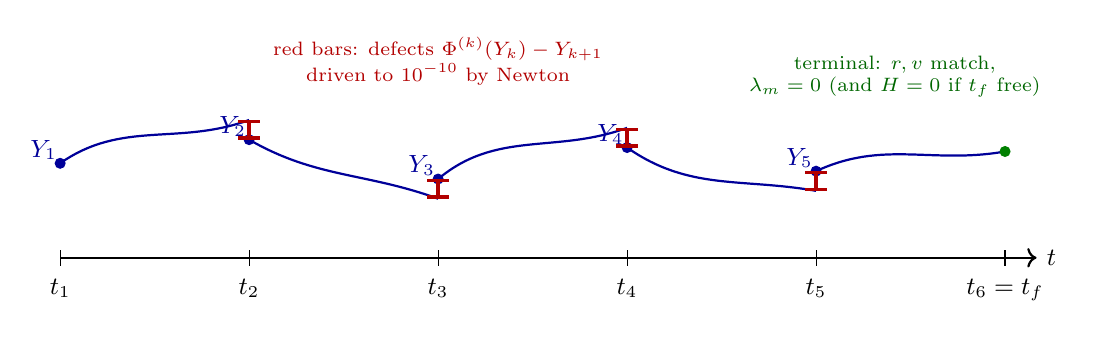
\begin{tikzpicture}[font=\small]
\draw[->,thick] (0,0)--(12.4,0) node[right]{$t$};
\foreach \k/\x/\y in {1/0/1.2,2/2.4/1.5,3/4.8/1.0,4/7.2/1.4,5/9.6/1.1} {
  \draw (\x,-0.1)--(\x,0.1); \node[below] at (\x,-0.15) {$t_{\k}$};
  \fill[blue!60!black] (\x,\y) circle (2pt);
  \node[above left,blue!60!black,inner sep=1pt] at (\x,\y) {$Y_{\k}$};
}
\draw (12,-0.1)--(12,0.1); \node[below] at (12,-0.15) {$t_6=\tf$};
\draw[thick,blue!60!black] (0,1.2)   to[out=35,in=200] (2.4,1.75);
\draw[thick,blue!60!black] (2.4,1.5) to[out=-30,in=160] (4.8,0.75);
\draw[thick,blue!60!black] (4.8,1.0) to[out=40,in=200] (7.2,1.65);
\draw[thick,blue!60!black] (7.2,1.4) to[out=-35,in=170] (9.6,0.85);
\draw[thick,blue!60!black] (9.6,1.1) to[out=25,in=190] (12,1.35);
\foreach \x/\a/\b in {2.4/1.75/1.5,4.8/0.75/1.0,7.2/1.65/1.4,9.6/0.85/1.1} {
  \draw[red!70!black,very thick,{Bar}-{Bar}] (\x,\a)--(\x,\b);
}
\fill[green!50!black] (12,1.35) circle (2pt);
\node[red!70!black,font=\scriptsize,align=center] at (4.8,2.5) {red bars: defects $\Phi^{(k)}(Y_k)-Y_{k+1}$\\driven to $10^{-10}$ by Newton};
\node[green!40!black,font=\scriptsize,align=center] at (10.6,2.3) {terminal: $r,v$ match,\\$\lm=0$ (and $H=0$ if $\tf$ free)};
\end{tikzpicture}
\caption{Multiple shooting: the arc is cut into $K$ segments; the junction states $Y_2,\dots,Y_K$ are unknowns along with the free part of $Y_1$ (the costates, and $\tf$ when free). Each segment is propagated only over its own short span, so the Lyapunov amplification that kills single shooting over 20--30 days (catalog seeds miss by 36,000--560,000 km when single-shot) never accumulates.}
\label{fig:ms}
\end{figure}

\begin{intu}
Single shooting integrates the whole arc from $y(0)$ and compares the endpoint
with the target: a root-finding problem in 7--8 unknowns whose Jacobian is a
product of state transition matrices over the entire flight --- and over
several revolutions of the Moon that product amplifies initial errors by
$10^3$--$10^4$. Newton then has a basin of attraction too small to hit from
any harvested seed. Multiple shooting adds the junction states as unknowns:
the problem gets bigger ($7+14(K-1)$ unknowns, $K=12$--$48$) but each residual
depends only on a \emph{short} propagation, the Jacobian is block-banded and
well-conditioned, and Newton converges from the collocation seed in 1--3
iterations. The price --- a bigger linear solve --- is trivial at this size.
\end{intu}

\begin{rig}
\textbf{Unknowns.} $p=[\,Y_1(\mathcal F);\ Y_2;\dots;Y_K;\ (\tf)\,]$ with $\mathcal F$ the
free rows of the first junction (the seven costates; the state part is fixed to
$[r_0;v_0;1]$). \textbf{Residual.}
\begin{equation}\label{eq:msres}
R(p)=\begin{bmatrix}\Phi^{(1)}(Y_1)-Y_2\\ \vdots\\ \Phi^{(K-1)}(Y_{K-1})-Y_K\\ g\big(\Phi^{(K)}(Y_K)\big)\end{bmatrix},
\qquad
g(y)=\begin{bmatrix} r-r_f\\ v-v_f\\ \lm\\ (H)\end{bmatrix},
\end{equation}
where $\Phi^{(k)}$ propagates segment $k$ over $\sigma_k\tf$ ($\sigma_k$ the fixed
normalized breakpoints) and the $H$ row exists only when $\tf$ is free.
\textbf{Jacobian.} Each segment's propagator returns its STM; the blocks are
$\partial R_k/\partial Y_k=\Phi_k$, $\partial R_k/\partial Y_{k+1}=-I$, and, for free
$\tf$, $\partial R_k/\partial\tf=\sigma_k f(y_{k+1}^-)$; the last block row is
$\partial g/\partial y\cdot\Phi_K$. \textbf{Solve.} \texttt{fsolve}
trust-region dogleg with the analytic Jacobian, then up to five plain Newton
polish steps (fsolve's first-order-optimality exit fires one step early on
short, well-conditioned arcs; measured). \textbf{Guards.} An iterate with a
non-finite entry, $\tf$ outside $[0.3,3]\times$ the seed, or $\|p\|_\infty>10^5$
is rejected with a large residual instead of being propagated (a wild iterate
can drive the integrator into collapse). Convergence: $\|R\|_\infty<10^{-10}$
(min-time) --- on 30-day fixed-$\tf$ arcs the residual floor is $\sim10^{-10}$ and
$3\times10^{-10}$ is used. The engine also reports $\operatorname{cond}(J)$ at
the final iterate (fold diagnosis) and, on request, the segment STMs and the
terminal state $y(\tf)$ for the second-order test.
\end{rig}

\begin{algorithm}[h]
\caption{\texttt{ms\_bvp}: generic multiple shooting (min-time and fixed-$\tf$)}
\begin{algorithmic}[1]
\Require problem closures \{prop, rhs, terminal\}, seed $\{\tf,\mathrm{tGrid},Y\}$, tolR
\State $p\gets[\,Y_1(\mathcal F);\,Y_{2:K};\,(\tf)\,]$; $\sigma\gets\mathrm{tGrid}/\tf$
\Function{residual}{$p$}
  \If{$p$ non-finite or outside the guards} \Return $R\gets 10^8\mathbf 1$, $J\gets I$ \EndIf
  \For{$k=1..K$} $[y^-_{k+1},\Phi_k]\gets\mathrm{prop}(\sigma_k\tf,\,Y_k)$ \Comment{one short propagation + STM}
    \State assemble block row $k$ of $R,J$ per \eqref{eq:msres}
  \EndFor
\EndFunction
\State $p\gets$ \texttt{fsolve}(residual, $p$, trust-region-dogleg, analytic $J$, wall budget)
\While{$\|R\|_\infty>$ tolR and polish steps $<5$} $p\gets p-J^{-1}R$ if it reduces $\|R\|_\infty$ \EndWhile
\State \Return $p$, info\{converged, normR, iters, condJ, junction states, $\Phi_k$ (optional), $y(\tf)$\}
\end{algorithmic}
\end{algorithm}

\subsection{Acceptance and the catalog}
\begin{intu}
A converged multiple-shooting solution is \emph{our} answer. The catalog's
consumer is pumpkyn's single-shooting \file{tfMin}. So the acceptance gate
is literally ``hand $z_8$ to \file{tfMin}; does it come back unchanged?''
--- PASS if $|\Delta z|<10^{-6}$ (observed $\sim10^{-9}$). That is a
\emph{foreign witness}: a different code, integrator and root finder agreeing
on the same seven numbers. It is the strongest first-order evidence in the
program and it exists only for min-time (pumpkyn has no min-fuel twin).
Catalogs are built by walking the thrust rungs 15 N $\to$ 0.5 N with warm
continuation on the $12\times12$ (or $6\times6$) phasing torus of each
(departure, arrival) sheet.
\end{intu}

\subsection{Verification of a min-time entry}\label{sec:mt-verify}
\begin{figure}[t]\centering
\resizebox{\textwidth}{!}{%
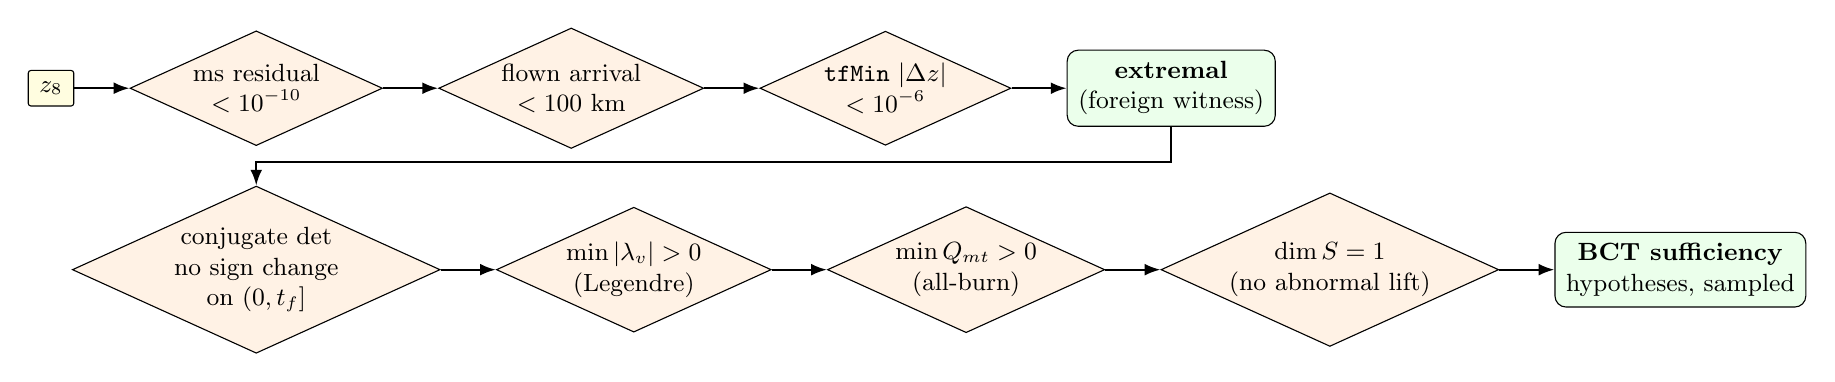
\begin{tikzpicture}[node distance=5mm and 7mm,font=\small]
\node[data] (z) {$z_8$};
\node[gate,right=of z] (g1) {ms residual\\$<10^{-10}$};
\node[gate,right=of g1] (g2) {flown arrival\\$<100$ km};
\node[gate,right=of g2] (g3) {\texttt{tfMin} $|\Delta z|$\\$<10^{-6}$};
\node[box,fill=green!8,right=of g3] (ext) {\textbf{extremal}\\(foreign witness)};
\node[gate,below=of g1] (c1) {conjugate det\\no sign change\\on $(0,\tf]$};
\node[gate,right=of c1] (c2) {$\min|\lv|>0$\\(Legendre)};
\node[gate,right=of c2] (c3) {$\min \Qmt>0$\\(all-burn)};
\node[gate,right=of c3] (c4) {$\dim S=1$\\(no abnormal lift)};
\node[box,fill=green!8,right=of c4] (loc) {\textbf{BCT sufficiency}\\hypotheses, sampled};
\draw[arr] (z)--(g1); \draw[arr] (g1)--(g2); \draw[arr] (g2)--(g3); \draw[arr] (g3)--(ext);
\draw[arr] (ext.south) |- ($(c1.north)+(0,3mm)$) -| (c1.north);
\draw[arr] (c1)--(c2); \draw[arr] (c2)--(c3); \draw[arr] (c3)--(c4); \draw[arr] (c4)--(loc);
\end{tikzpicture}}
\caption{What a min-time entry has passed. Top row: level 1, the Pontryagin extremal --- every catalog entry. Bottom row: level 2, local minimality --- the hypotheses of the Bonnard--Caillau--Tr\'elat sufficiency theorem, checked numerically by \texttt{conj\_catalog\_pass} and \texttt{gates\_catalog\_pass} (the determinant is sampled at junctions, so this is an assessment, not a proof --- \S\ref{sec:proves}).}
\label{fig:mt-verify}
\end{figure}

\begin{eli}
Being a root of the equations only means the trajectory is a \emph{candidate}
--- a hilltop and a valley bottom both have zero slope. To know it is a valley
we look at the second derivative, which for trajectories means: does a nearby
trajectory that starts at the same place and satisfies the same equations
come back and touch this one somewhere in the middle? If it does (a
\emph{conjugate point}), the trajectory is not the shortest; think of two great
circles from the north pole meeting again at the south pole --- past the south
pole, the arc is no longer shortest.
\end{eli}

\begin{intu}
The Jacobi field is the linearized effect on the state of perturbing the
initial costate: $\delta x(t)=\Phi_{x\lambda}(t,0)\,\delta\lambda(0)$. A
conjugate time is where some nonzero $\delta\lambda(0)$ produces
$\delta x(t)=0$ --- the linearized endpoint map loses rank. For min-time two
exact degeneracies must be removed first or the determinant is identically
zero: the control depends only on the \emph{direction} of $\lv$, so scaling
$\lambda(0)$ changes nothing ($\Phi_{x\lambda}\lambda(0)=0$ exactly), and $\lm$
never enters the control (its column is zero). The instrument therefore
projects out $\lambda(0)$ (columns $P$ spanning its complement) and appends
the flow direction $f$ (free time). \emph{This quotient is proven equivalent
to the Bonnard--Caillau--Tr\'elat construction on the $H=0$ slice}
(\file{doc/mintime\_second\_order\_audit.tex}, image-space lemma).
\end{intu}

\begin{rig}
\textbf{Instrument} (\file{ms\_conjugate\_test}, free-time form): with the
segment STMs from the converged solve, $\Phi(t_{k+1},0)=\Phi_k\cdots\Phi_1$,
\[
D(t_{k+1})=\det\big[\,\Phi_{rv,\lambda_{rv}}(t_{k+1},0)\,P,\ \ f_{rv}(y(t_{k+1}))\,\big]\in\R^{6\times6},\qquad k=1..K,
\]
sampled through $\tf$ (the terminal state comes from the engine). The block is
equilibrated (positive row/column scaling, sign-safe), the sign is taken from a
pivoted LU, the magnitude kept as a log-determinant (an underflowing raw det can
never read as a root). Samples before the state block first attains full rank
(an initial coast or saturated arc: structurally zero, not a focal point) are
skipped. Verdict: FAIL if a sign change (or an isolated zero run) lies strictly
before the last bracket; ENDPOINT if the only root is on the bracket ending
at $\tf$ (a weak, non-strict minimum --- examine, do not refute); UNDETERMINED
if nothing was testable; PASS otherwise.
\textbf{Hypothesis gates} (\file{mintime\_hypothesis\_gates}, on the dense
\file{tfMinProp} flight): $\min_t|\lv|>0$ (strong Legendre,
$H_{\alpha\alpha}|_{TS^2}=\frac{T}{m}|\lv|I$); $\min_t \Qmt>0$ with
$\Qmt=|\lv|/m+\lm/c$ (the all-burn assumption is the PMP control; this is
\file{tfMinEoM}'s own switching function); and the abnormal-lift probe: lifts of
a fixed trajectory form a linear space $S=\{\lambda:\dot\lambda=-A(t)^{\!\top}\lambda,\ \lv\parallel\alpha(t),\ \lm(\tf)=0\}$
with $A$ the fixed-control Jacobian; $\lambda\cdot f$ is a linear functional on
$S$ whose kernel is the abnormal lifts; our normal lift has $\lambda\cdot f=-1$,
so \emph{no abnormal lift exists iff $\dim S=1$}, computed as $7-\operatorname{rank}C$
for the stacked constraint matrix $C$, with the rank threshold tied to the
accuracy of the known member: $\mathrm{tol}=\min(\max(10^{-8}\sigma_1,\,10\,\|C\lambda_0\|/\|\lambda_0\|),\,10^{-3}\sigma_1)$
(a null space cannot be resolved finer than its known member's residual; a
fixed $10^{-8}$ under-counted 512 entries as ``$\dim S=0$'' on the first pass).
\textbf{Status.} Conjugate test: 18,249 entries PASS / 61 refuted / 50
unverified on the (pre-09-05) instrument; the corrected instrument reproduces
the 20 golden verdicts. Gates: 18,360/18,360 pass, written into the catalogs
as \texttt{gate\_min\_lamv}, \texttt{gate\_min\_qmt}, \texttt{gate\_dimS};
spectral gap $\sigma_7/\sigma_6\le2.5\times10^{-6}$ everywhere; $\min|\lv|$
falls with thrust (593 entries below $10^{-4}$, all at $\ge2$ N) --- the
high-thrust primer near-nulls are where a strict certificate will be hardest.
\end{rig}

\begin{warn}
\textbf{Defect $\ne$ accuracy}\label{sec:defect}: a collocation solution with
defects $10^{-14}$ can have a true continuous-time local error of 1441 km
(trapezoid, $N=800$, DRO$\to$tulip); Hermite--Simpson at $N=1600$ reaches
3 m. The indirect solution is what is certified; the direct one is the seed.
\textbf{The determinant is sampled} at $K$ junctions: a conjugate pair inside
one segment or an even-multiplicity root is invisible. \textbf{Normality}:
\file{tfMin} acceptance gives a normal lift; exclusivity is the $\dim S$ gate.
\end{warn}

%======================================================================
\section{Min-fuel: from min-energy by homotopy}
%======================================================================

\begin{figure}[t]\centering
\resizebox{\textwidth}{!}{%
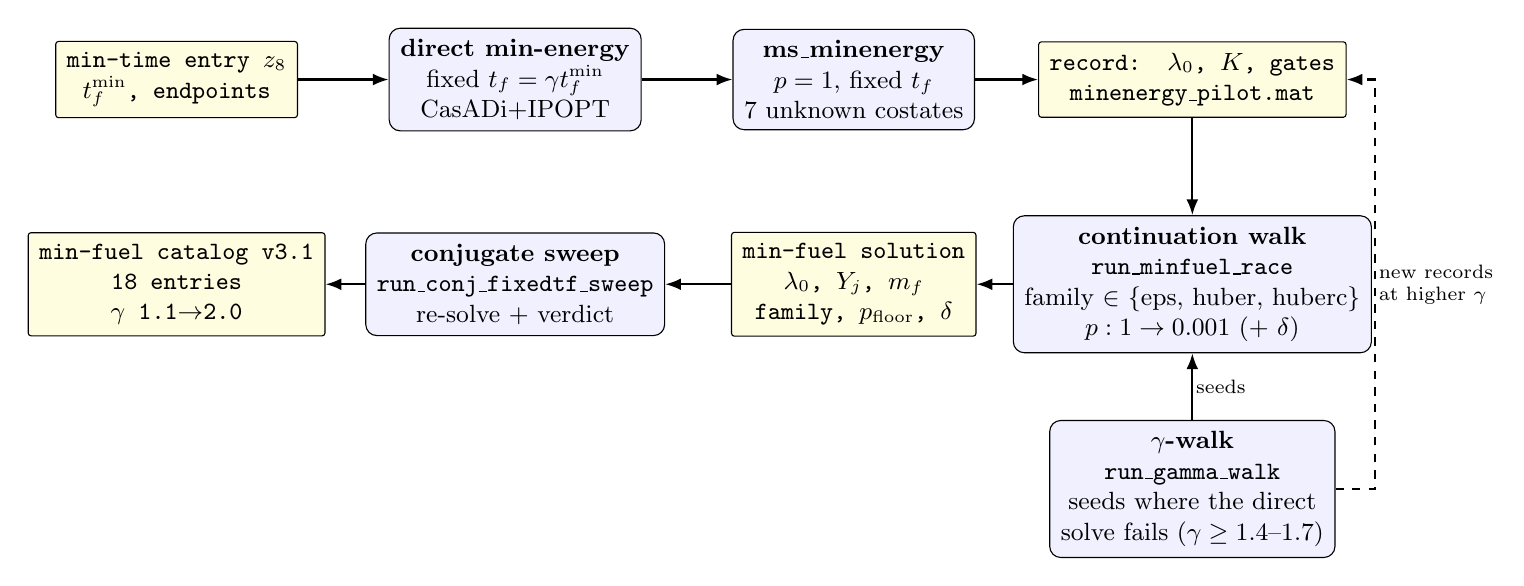
\begin{tikzpicture}[font=\small]
\node[data] (mt) at (0,0) {min-time entry $z_8$\\$\tf^{\min}$, endpoints};
\node[proc] (dir) at (4.3,0) {\textbf{direct min-energy}\\fixed $\tf=\gamma\tf^{\min}$\\CasADi+IPOPT};
\node[proc] (msE) at (8.6,0) {\textbf{ms\_minenergy}\\$p=1$, fixed $\tf$\\7 unknown costates};
\node[data] (rec) at (12.9,0) {record: $\lambda_0$, $K$, gates\\\file{minenergy\_pilot.mat}};
\node[proc] (walk) at (12.9,-2.6) {\textbf{continuation walk}\\\texttt{run\_minfuel\_race}\\family $\in$ \{eps, huber, huberc\}\\$p:1\to0.001$ (+ $\delta$)};
\node[data] (fuel) at (8.6,-2.6) {min-fuel solution\\$\lambda_0$, $Y_j$, $m_f$\\family, $p_{\rm floor}$, $\delta$};
\node[proc] (sweep) at (4.3,-2.6) {\textbf{conjugate sweep}\\\texttt{run\_conj\_fixedtf\_sweep}\\re-solve + verdict};
\node[data] (cat) at (0,-2.6) {\textbf{min-fuel catalog} v3.1\\18 entries\\$\gamma$ 1.1$\to$2.0};
\node[proc] (gw) at (12.9,-5.2) {\textbf{$\gamma$-walk}\\\texttt{run\_gamma\_walk}\\seeds where the direct\\solve fails ($\gamma\ge1.4$--$1.7$)};
\draw[arr] (mt)--(dir); \draw[arr] (dir)--(msE); \draw[arr] (msE)--(rec); \draw[arr] (rec)--(walk);
\draw[arr] (walk)--(fuel); \draw[arr] (fuel)--(sweep); \draw[arr] (sweep)--(cat);
\draw[arr] (gw)--node[lbl,right]{seeds}(walk);
\draw[arr,dashed] (gw.east) -- ++(0.5,0) |- node[lbl,pos=0.25,right,align=left]{new records\\at higher $\gamma$} (rec.east);
\end{tikzpicture}}
\caption{The min-fuel line. The min-energy problem at fixed $\tf$ is the smooth entry point; a continuation in the smoothing parameter $p$ deforms it into min-fuel. Where the direct min-energy solve fails (high $\gamma$), a continuation in $\tf$ itself supplies the seed.}
\label{fig:mf-pipeline}
\end{figure}

\subsection{Why not solve min-fuel directly?}
\begin{eli}
Newton's method steers by slopes. A bang-bang throttle is a step function ---
no slope anywhere, and infinite slope at the switch. Aim Newton at it cold and
it has nothing to hold on to. So we cheat: we solve a \emph{softened} problem
where the throttle is a gentle ramp instead of a step, and then, like cooling
butter a little at a time, sharpen the ramp step by step, using each answer
as the guess for the next. That is a \emph{homotopy}. The dial that sets the
sharpness is $p$.
\end{eli}

\subsection{The three smoothing families}\label{sec:families}
\begin{figure}[t]\centering
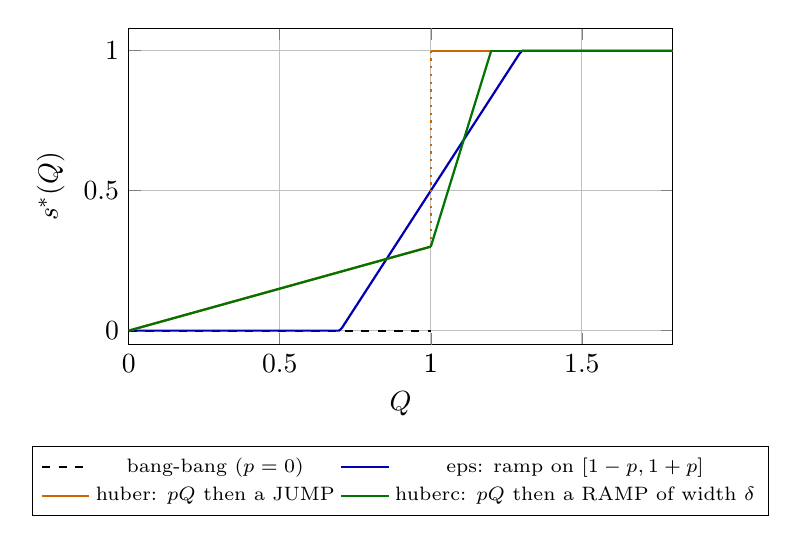
\begin{tikzpicture}
\begin{axis}[width=0.7\textwidth,height=5.6cm,xlabel={$Q$},ylabel={$s^*(Q)$},xmin=0,xmax=1.8,ymin=-0.05,ymax=1.08,
  legend style={at={(0.5,-0.32)},anchor=north,font=\scriptsize},legend columns=2,grid=major,
  extra x ticks={1},extra x tick labels={$1$},extra x tick style={grid=none}]
\addplot[black,dashed,thick,samples=2,domain=0:0.999] {0};
\addlegendentry{bang-bang ($p=0$)}
\addplot[black,dashed,thick,samples=2,domain=1.001:1.8,forget plot] {1};
\addplot[blue!70!black,thick,domain=0:1.8,samples=200] {min(max((x-(1-0.3))/(2*0.3),0),1)};
\addlegendentry{eps: ramp on $[1-p,1+p]$}
\addplot[orange!80!black,thick,domain=0:0.999,samples=50] {0.3*x};
\addlegendentry{huber: $pQ$ then a JUMP}
\addplot[orange!80!black,thick,domain=1.001:1.8,samples=2,forget plot] {1};
\addplot[orange!80!black,thick,dotted,samples=2,forget plot] coordinates {(1,0.3) (1,1)};
\addplot[green!45!black,thick,domain=0:1,samples=50] {0.3*x};
\addlegendentry{huberc: $pQ$ then a RAMP of width $\delta$}
\addplot[green!45!black,thick,domain=1:1.2,samples=20,forget plot] {0.3+(1-0.3)*(x-1)/0.2};
\addplot[green!45!black,thick,domain=1.2:1.8,samples=2,forget plot] {1};
\end{axis}
\end{tikzpicture}
\caption{Throttle law $s^*=\arg\min_{[0,1]}(L(s)-sQ)$ for the three families at $p=0.3$ ($\delta=0.2$ for huberc). All three tend to the bang-bang step as $p\to0$; they differ in \emph{how} the step is approached --- and that difference decides where Newton walks and where it walls.}
\label{fig:families}
\end{figure}

\begin{rig}
Each family is a running cost $L(s)$; the throttle law is its exact argmin
(verified numerically to $10^{-16}$ in $H$ for all three):
\[
\begin{array}{lll}
\text{eps (Bertrand--Epenoy)} & L=(1-p)s+ps^2 & s^*=\mathrm{clip}\big(\tfrac{Q-(1-p)}{2p},0,1\big)\\[2pt]
\text{huber (PLQ)} & L=\begin{cases}s^2/2p & s\le p\\ s-p/2 & s>p\end{cases} & s^*=\begin{cases}pQ&Q<1\\ 1&Q>1\end{cases}\ \text{(jump at }Q=1)\\[8pt]
\text{huberc (hybrid)} & L=\begin{cases}s^2/2p & s\le p\\ \tfrac p2+(s-p)+\tfrac{\delta(s-p)^2}{2(1-p)} & s>p\end{cases} & s^*=\begin{cases}pQ&Q<1\\ p+(1-p)\tfrac{Q-1}{\delta}&1\le Q<1+\delta\\ 1&Q\ge1+\delta\end{cases}
\end{array}
\]
At $p=1$, eps \emph{is} the min-energy field (exactly, dF $=0$); huber and
huberc at $p=1$ give $s^*=\mathrm{clip}(Q,0,1)$ --- the same trajectory as
min-energy but with costates halved (\S\ref{sec:seed}). At $p\to0$ all three
tend to the bang-bang law. huberc is $C^0$ in $Q$ with $L$ strictly convex
($L''>0$ on both pieces, $C^1$ at $s=p$), so its argmin is unique; $\delta\to0$
recovers huber.
\end{rig}

\begin{intu}
Why three? eps was the original convention: it works everywhere, slowly
(8--10 failed rungs per walk near the floor, where its ramp slope $1/2p$ reaches
$\sim400$). Huber was proposed as a PLQ alternative and \emph{appeared} to fail
structurally --- until the review found that its jump had been propagated
without the saltation matrix (\S\ref{sec:saltation}); with that fixed it is the
\emph{fastest} family by $5\times$ and failure-free where it works, because
below the jump its slope is $p$, gentle and getting gentler. But it walls on
$\sim30\%$ of cells, and the wall has a signature: a switch about to be born or
annihilated at a tangency of $Q$ with 1 (a grazing-risk structure change), where
the trajectory map is not smooth in the unknowns. huberc keeps Huber's gentle
core and replaces the jump with a short ramp of width $\delta$: continuous
$\Rightarrow$ no corner $\Rightarrow$ it passed both Huber walls --- and, when
$\delta$ is held fixed at $\sim0.03$ during the $p$-walk, that walk is
failure-free; the sharpening of $\delta$ afterwards costs what every family pays
at the floor, and by then $m_f$ has converged to $10^{-6}$.
\end{intu}

\subsection{The seed and the walk}\label{sec:seed}
\begin{rig}
\textbf{Seed.} A min-energy record stores $\lambda_0$ and $K$; the walk rebuilds
the $K{+}1$ junction states by flying the energy field from $[r_0;v_0;1;\lambda_0]$
and sampling the uniform breakpoints. For the Huber families the costates are
halved: at $p=1$ their minimizer is $s^*=Q$, the energy law's is $Q/2$, so
$\lambda/2$ reproduces the same trajectory (measured: the $p=1$ rung then
converges in 2 Newton iterations; with the unscaled seed one 30-day cell failed
its first rung cold).
\textbf{Rung.} At each $(p,\delta)$: \file{ms\_minfuel} = \file{ms\_bvp} with
fixed $\tf$, unknowns $[\lambda_0;Y_{2:K}]$, terminal $g=[r-r_f;v-v_f;\lm]$,
propagator \file{cr3bp\_minfuel\_prop} in the current family; accept when
converged ($\|R\|_\infty<3\times10^{-10}$) and $|H(t_k)-H(t_1)|<10^{-6}$ at the
junctions ($H$ is a first integral at fixed $\tf$); the accepted junctions
(plus the last segment propagated to $\tf$) seed the next rung.
\textbf{Failure.} Geometric bisection toward the last good $p$ (up to
\texttt{maxBisect} inserts), two abandoned gaps retire the arm. The deepest
accepted rung is the arm's answer; $m_f$ is read from the arm's own flight of
its own solution.
\textbf{Two-stage schedule (huberc).} Stage 1 walks $p$ with $\delta$ from a
rule (fixed 0.03 recommended); stage 2 holds $p$ at its floor and walks $\delta$
down (0.02 $\to$ 0.003). Loose-rung acceptance (MfMax's \texttt{homCI} idea,
$\|R\|<10^{-3}$ with the floor refined to full tolerance) is available and was
measured \emph{not} to pass the Huber walls.
\end{rig}

\begin{algorithm}[h]
\caption{\texttt{run\_minfuel\_race}: one continuation arm}
\begin{algorithmic}[1]
\Require min-energy record, family, schedule $p_1{=}1>p_2>\dots>p_n$, $\delta$ rule, seedScale
\State seed $\gets$ fly $\lambda_0$ with the energy field, cut at $K{+}1$ breakpoints; scale costates by seedScale
\State queue $\gets\{(p_i,\delta(p_i))\}$; \ good $\gets\varnothing$; gaps $\gets0$
\While{queue not empty}
  \State $(p,\delta)\gets$ pop; $[\lambda_0,\mathrm{info}]\gets$ \texttt{ms\_minfuel}(seed, family, $p$, $\delta$) \Comment{hard-capped worker}
  \If{converged and $H$-drift $<10^{-6}$}
     \State record rung ($m_f$ from the flown solution, coast fraction, cond$J$); seed $\gets$ junctions; good $\gets p$
  \ElsIf{good $\ne\varnothing$ and bisection budget left} push $(\sqrt{\text{good}\cdot p},\cdot)$ then $(p,\cdot)$ back
  \Else\ gaps $\gets$ gaps$+1$; retire if gaps $=2$
  \EndIf
\EndWhile
\State optional stage 2: hold $p$, walk $\delta$ down with the same loop
\State refine the floor to full tolerance; run the single-shooting acceptance probe (advisory at deep $p$)
\end{algorithmic}
\end{algorithm}

\subsection{The Huber jump and the saltation matrix}\label{sec:saltation}
\begin{eli}
Roll a marble down a ramp and ask how far the landing spot moves if you nudge
the start. On a smooth ramp, follow the slope. But if the ramp has a
\emph{step}, the marble flies off the edge, and a nudge at the start changes
\emph{when} it reaches the edge --- which moves the landing spot a lot.
Following the local slope alone misses that. Our Huber throttle has a step at
$Q=1$; the sensitivity matrix Newton needs must include the step.
\end{eli}
\begin{rig}
At a crossing of the switch surface $h(y)=Q(y)-1=0$ with incoming field $F^-$
and outgoing $F^+$, the state transition matrix receives the jump
\begin{equation}\label{eq:salt}
\Phi^+=\Big[I+\frac{(F^+-F^-)\,n^{\!\top}}{n^{\!\top}F^-}\Big]\Phi^-,\qquad n=\nabla_y Q,
\end{equation}
implemented by event-split propagation: integrate each smooth branch with the
law pinned, stop at the event, apply \eqref{eq:salt}, restart on the other
branch. Two facts make this clean. (i) $n^{\!\top}F$ is $\dot Q$, and for this
Hamiltonian the throttle drops out of $\dot Q$ exactly,
\[
\dot Q=-\,\frac{T\,\lv^{\!\top}\lr}{m\,|\lv|}\qquad(\text{measured } n^{\!\top}(F^+-F^-)=9\times10^{-16}),
\]
so the denominator is continuous across the switch and is computed in closed
form (\file{cr3bp\_minfuel\_qdot}); it is also the exact transversality of the
crossing --- the grazing diagnostic. (ii) For the continuous families (eps,
huberc) $F^+=F^-$ at every branch boundary, the bracket is the identity, and
the branchwise-AD STM \emph{is} the derivative of the flow: no saltation needed.
Measured against finite differences across one switch: Huber STM error
$1.35\times10^{-3}$ without \eqref{eq:salt}, $2.1\times10^{-6}$ with (the harness
floor, $1.35\times10^{-7}$ on eps).
\end{rig}
\begin{warn}
Without \eqref{eq:salt} the Huber arm looked ``structurally unsuited'' (2 rungs,
8 fails); with it the same cell walks 17/17 rungs with 0 fails. A wrong Jacobian
and a hard wall look identical from the outside --- check the map against
finite differences before declaring a method unsuited (\file{test\_huber\_saltation}
is the standing test). At a \emph{grazing} crossing ($\dot Q\to0$) the bracket
blows up; the propagator refuses (assert) rather than silently continuing.
\end{warn}

\subsection{Seeds where the direct solver fails: the $\gamma$-walk}
\begin{intu}
For $\gamma\ge1.7$ on one cell and $\ge1.4$ on the others the direct
min-energy NLP does not converge, so the fuel line had no seed there. But
min-energy is smooth, and multiple shooting continues happily in the
\emph{boundary data}: take the deepest converged record, stretch its junction
states to the new, longer time grid at the same fractional times, and re-solve;
bisect $\gamma$ on failure. This is MfMax's initial-condition homotopy in the
form the program already trusted. It opened one cell to $\gamma=2$ in three
minutes, every step conjugate-tested, and located two \emph{smooth} walls
($\gamma\approx1.43$ and $1.27$) where cond$(J)$ grows by two orders on approach
--- a fold signature, the first real candidate for pseudo-arclength continuation.
\end{intu}

\subsection{Verification of a min-fuel entry}
\begin{figure}[t]\centering
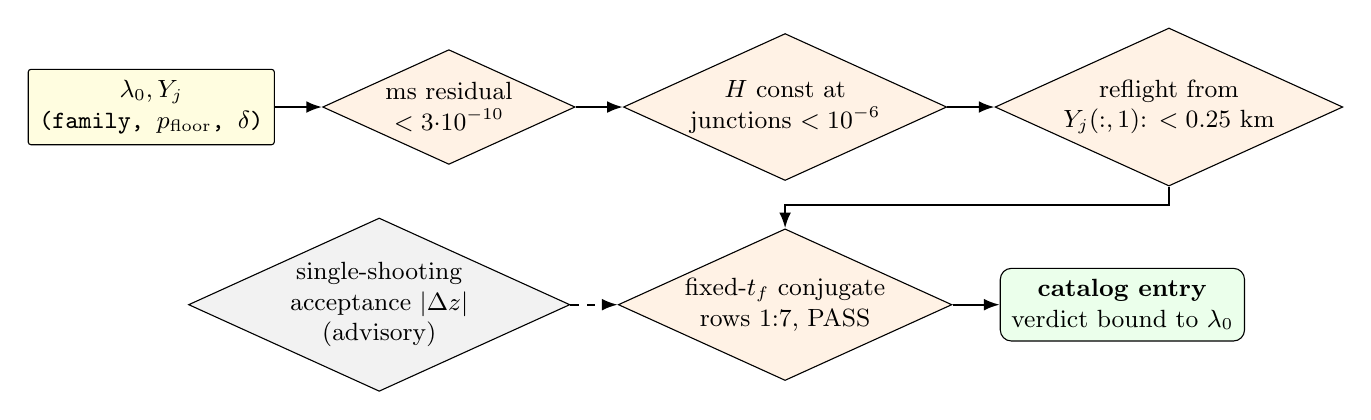
\begin{tikzpicture}[node distance=6mm and 6mm,font=\small]
\node[data] (s) {$\lambda_0,Y_j$\\(family, $p_{\rm floor}$, $\delta$)};
\node[gate,right=of s] (g1) {ms residual\\$<3{\cdot}10^{-10}$};
\node[gate,right=of g1] (g2) {$H$ const at\\junctions $<10^{-6}$};
\node[gate,right=of g2] (g3) {reflight from\\$Y_j(:,1)$: $<0.25$ km};
\node[gate,below=of g2] (g4) {fixed-$\tf$ conjugate\\rows 1:7, PASS};
\node[box,fill=green!8,right=of g4] (out) {\textbf{catalog entry}\\verdict bound to $\lambda_0$};
\node[gate,left=of g4,fill=gray!10] (ss) {single-shooting\\acceptance $|\Delta z|$\\(advisory)};
\draw[arr] (s)--(g1); \draw[arr] (g1)--(g2); \draw[arr] (g2)--(g3);
\draw[arr] (g3.south) |- ($(g4.north)+(0,3mm)$) -| (g4.north);
\draw[arr] (g4)--(out);
\draw[arr,dashed] (ss)--(g4);
\end{tikzpicture}
\caption{What a min-fuel entry has passed. Level 1: multiple-shooting residual, first-integral conservation, and the deliverable's own reconstruction recipe. Level 2: the fixed-$\tf$ Jacobi necessary condition on the full-state block. The single-shooting acceptance probe is advisory only at deep $p$: single shooting over 20--30 days wanders even from a true root (FINDINGS 19) --- 6 of 7 grid entries fail it while reflying to $<0.15$ km.}
\label{fig:mf-verify}
\end{figure}

\begin{rig}
\textbf{Level 1.} The ms residual and $H$ conservation certify the extremal;
the reflight (fly \file{cr3bp\_minfuel\_prop} from $Y_j(:,1)$ over $\tf$ in the
entry's own family) certifies the deliverable's recipe --- worst 0.22 km over
the 18 entries. There is no foreign witness for min-fuel (pumpkyn has no twin;
MfMax is two-body). \textbf{Level 2.} \file{ms\_conjugate\_test} in its
fixed-$\tf$ form: no flow column, no quotient (the running cost breaks the
scaling invariance), rows $1{:}7$ --- the FULL state, mass included: an interior
conjugate point is a Jacobi field vanishing in $r,v$ \emph{and} $m$, because only
then does its zero-extension give an admissible variation. (The mixed block
$[1{:}6\ 14]$ used until 2026-09-05 is the terminal shooting Jacobian, meaningful
only at $\tf$; the one ``refutation'' it produced was an initial-coast
structural zero.) For the continuous families the branchwise-AD STM is the
true flow derivative at transversal band crossings, so this is the ordinary
Jacobi necessary condition; for huber entries the saltation STMs are used.
\textbf{Binding.} \file{run\_conj\_fixedtf\_sweep} re-solves every packaged
solution in its own family with STMs kept and stores the verdict with the
$\lambda_0$, $p$, family and rows it was computed on; \file{build\_minfuel\_catalog}
refuses any verdict that does not match the entry. Current: 26/26 PASS, all
tested, none endpoint-only.
\end{rig}
\begin{warn}
The catalog entries are solutions of the \emph{smoothed} problem at
$p_{\rm floor}\approx10^{-3}$ (ramp width $\sim0.002$--$0.009$), not of the exact
bang-bang problem; $m_f$ has converged to $\sim10^{-6}$ by then, switch times
may still differ. Sufficiency for the fixed-$\tf$ free-mass problem needs the
terminal-manifold (focal/backward-Riccati) construction, not built; the
interior test is necessary-only. Below ramp width $\sim0.003$ every family
stalls on this solver configuration --- past that the problem is a
switching-time problem with fixed structure, which is the natural endgame and
the same build as a strict certificate (Maurer--Osmolovskii).
\end{warn}

%======================================================================
\section{Data flow, end to end}
%======================================================================
\begin{figure}[t]\centering
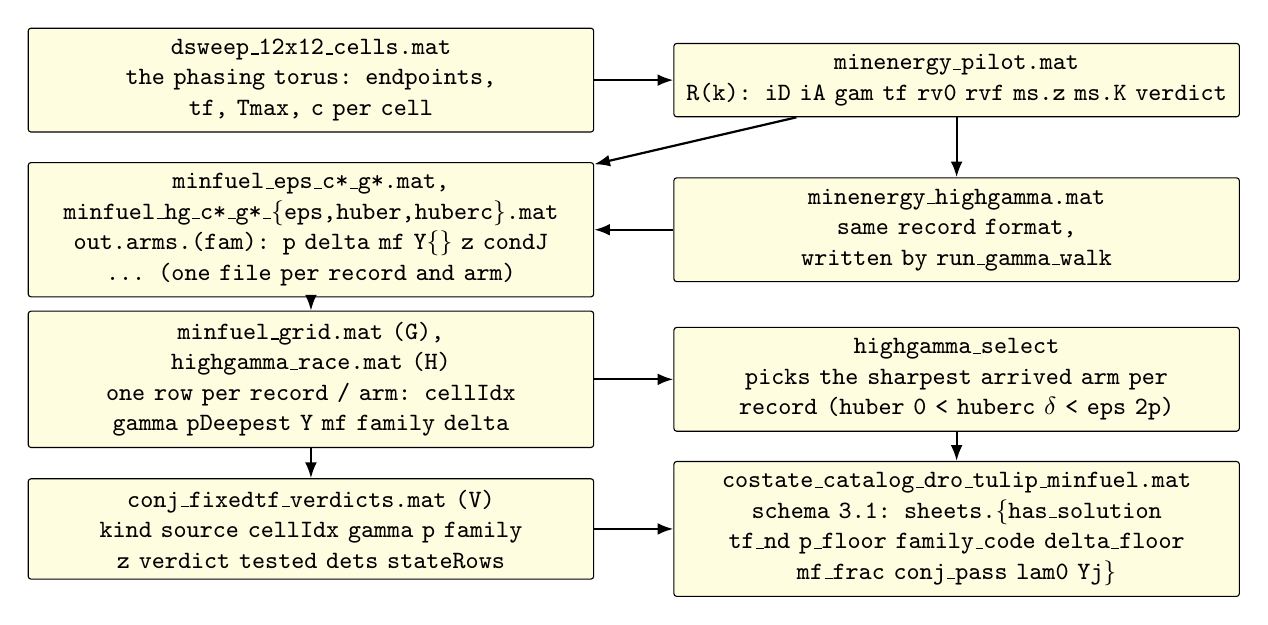
\begin{tikzpicture}[font=\scriptsize\ttfamily, every node/.append style={text width=6.9cm}]
\node[data] (a) at (0,0) {dsweep\_12x12\_cells.mat\\the phasing torus: endpoints, tf, Tmax, c per cell};
\node[data] (b) at (8.2,0) {minenergy\_pilot.mat\\R(k): iD iA gam tf rv0 rvf ms.z ms.K verdict};
\node[data] (c) at (8.2,-1.9) {minenergy\_highgamma.mat\\same record format, written by run\_gamma\_walk};
\node[data] (d) at (0,-1.9) {minfuel\_eps\_c*\_g*.mat, minfuel\_hg\_c*\_g*\_\{eps,huber,huberc\}.mat\\out.arms.(fam): p delta mf Y\{\} z condJ ... (one file per record and arm)};
\node[data] (e) at (0,-3.8) {minfuel\_grid.mat (G), highgamma\_race.mat (H)\\one row per record / arm: cellIdx gamma pDeepest Y mf family delta};
\node[data] (h) at (8.2,-3.8) {highgamma\_select\\picks the sharpest arrived arm per record (huber 0 < huberc $\delta$ < eps 2p)};
\node[data] (f) at (0,-5.7) {conj\_fixedtf\_verdicts.mat (V)\\kind source cellIdx gamma p family z verdict tested dets stateRows};
\node[data] (g) at (8.2,-5.7) {costate\_catalog\_dro\_tulip\_minfuel.mat\\schema 3.1: sheets.\{has\_solution tf\_nd p\_floor family\_code delta\_floor mf\_frac conj\_pass lam0 Yj\}};
\draw[arr] (a)--(b); \draw[arr] (b)--(c); \draw[arr] (b)--(d); \draw[arr] (c)--(d); \draw[arr] (d)--(e);
\draw[arr] (e)--(f); \draw[arr] (f)--(g); \draw[arr] (e)--(h); \draw[arr] (h)--(g);
\end{tikzpicture}
\caption{Files of the fixed-$\tf$ line and what each carries. Everything downstream of a record is reproducible from the record's $\lambda_0$ and $K$ (or, for min-fuel, from $Y_j$ --- the identifiability rule: at deep $p$ the junctions, not $\lambda_0$ alone, identify the solution).}
\label{fig:files}
\end{figure}

\begin{eli}
Think of three shelves. Top shelf: the min-energy records --- one per
(cell, $\gamma$), each a starting point. Middle shelf: the walks --- for each
record and each family, the whole ladder of solutions down to the floor. Bottom
shelf: the catalog --- one chosen solution per record, with its verdict stapled
to it and the proof that the verdict was computed on \emph{that} solution.
\end{eli}

%======================================================================
\section{What is proven, what is assessed}\label{sec:proves}
%======================================================================
\begin{center}\small
\begin{tabular}{@{}lp{0.42\textwidth}p{0.38\textwidth}@{}}
\toprule
claim & min-time entry & min-fuel entry \\
\midrule
PMP extremal & ms residual $10^{-10}$; \textbf{foreign witness} (\texttt{tfMin}) to $|\Delta z|\sim10^{-9}$ & ms residual $3\!\times\!10^{-10}$, $H$ const, reflight; \emph{no foreign witness} \\
no interior conjugate point & BCT determinant (proven equivalent to the theorem's construction), sampled at $K$ junctions & fixed-$\tf$ full-state determinant, sampled; necessary condition only \\
sufficiency hypotheses & $\min|\lv|>0$, $\min\Qmt>0$, $\dim S=1$ --- gated, 18,360/18,360 pass & not applicable in this form (mixed bang / interior arcs; needs the terminal-manifold focal test) \\
what a PASS licenses & ``normal extremal, no abnormal lift, strong Legendre and all-burn hold along the arc, no sign change of the BCT determinant at the sampled times'' & ``extremal of the smoothed problem at $p_{\rm floor}$, reflies to $<0.25$ km, no interior conjugate point at junction resolution'' \\
not claimed & strict local minimality as a theorem (sampling); global optimality & bang-bang optimality (finite $p$); local minimality \\
\bottomrule
\end{tabular}
\end{center}

%======================================================================
\section{Known walls and where the algorithms go next}
%======================================================================
\begin{itemize}
\item \textbf{Huber walls} (grazing-risk switch-structure changes): cured by
huberc; a family schedule --- Huber for speed, huberc at a predicted graze
(\file{huber\_switch\_diag}: $\min|\dot Q|$ at crossings, extrema of $Q$ near 1),
eps as the fallback --- is the reading of every table since \S\ref{sec:families}.
\item \textbf{Smooth walls in $\gamma$} (1.43 on (6,8), 1.27 on (1,2)): cond$(J)$
blows up on approach; no throttle family can help (no switch structure at
$p=1$); pseudo-arclength in \file{ms\_bvp} ($\partial F/\partial\tf$ is available)
is the candidate.
\item \textbf{The floor} (ramp width $\lesssim0.003$): a switching-time Newton
with fixed structure, which is also the strict second-order certificate.
\item \textbf{Deep thrust} (0.09 $\to$ 0.067 N): a basin wall at $\sim1.3$ revs,
needs a winding-aware route.
\end{itemize}

\section*{Glossary}
\begin{tabular}{@{}ll@{}}
$Q$ & switch quantity $T(|\lv|/m+\lm/c)$; fuel law switches at $Q=1$ \\
$\Qmt$ & $|\lv|/m+\lm/c$; min-time all-burn condition $\Qmt>0$ \\
$p$, $\delta$ & smoothing parameter (all families), ramp width (huberc) \\
$\gamma$ & $\tf/\tf^{\min}$ \\
$K$ & multiple-shooting segment count (12 fixed-$\tf$; 24--48 min-time) \\
$z_8$, $\lambda_0$, $Y_j$ & min-time entry; fixed-$\tf$ initial costate; junction states \\
$\Phi$ & state transition matrix of the 14-state PMP flow \\
saltation & the STM jump \eqref{eq:salt} at a control discontinuity \\
conjugate point & first time the linearized endpoint map loses rank \\
\end{tabular}

\section*{References}
\begin{itemize}
\item Bertrand \& Epenoy, ``New smoothing techniques for solving bang-bang optimal control problems,'' OCAM 23 (2002).
\item Bonnard, Caillau, Tr\'elat, ``Second order optimality conditions in the smooth case and applications in optimal control,'' ESAIM: COCV 13 (2007).
\item Betts, \emph{Practical Methods for Optimal Control Using Nonlinear Programming}, SIAM (2010), ch.~3 (multiple shooting).
\item Hairer, N\o rsett, Wanner, \emph{Solving ODEs I}, II.6 (sensitivity across a discontinuity).
\item Rockafellar \& Wets, \emph{Variational Analysis} (1998), PLQ penalties.
\item Osmolovskii \& Maurer, \emph{Applications to Regular and Bang-Bang Control}, SIAM (2012).
\item Code and record: \file{orbit\_transfer/costate\_common/}, \file{DRO\_tulip/FINDINGS.md} \S17--29, \file{doc/mintime\_second\_order\_audit.tex}, \file{doc/extremal\_and\_local\_min\_survey.md}, \file{doc/mfmax\_ideas\_review.md}.
\end{itemize}
\end{document}
